\documentclass[11pt, oneside]{article}   	% use "amsart" instead of "article" for AMSLaTeX format

\usepackage{geometry}
 \geometry{
 a4paper,
 total={170mm,257mm},
 left=20mm,
 top=30mm,
 bottom=25mm, 
 }
 
%\usepackage{geometry}                		% See geometry.pdf to learn the layout options. There are lots.
%\geometry{letterpaper}                   		% ... or a4paper or a5paper or ... 
%\geometry{landscape}                		% Activate for rotated page geometry
%\usepackage[parfill]{parskip}    		% Activate to begin paragraphs with an empty line rather than an indent
\usepackage{graphicx}				% Use pdf, png, jpg, or eps§ with pdflatex; use eps in DVI mode
								% TeX will automatically convert eps --> pdf in pdflatex		

\usepackage{amssymb}
\usepackage{amsmath}
\usepackage{amsthm}
\usepackage{fancyhdr}
\usepackage[utf8]{inputenc}
\usepackage[english]{babel}
\usepackage{enumerate}
\usepackage{arcs}
\usepackage{array}
\usepackage{tabularx} 
\usepackage{tikz}
%SetFonts

%SetFonts

\usepackage[inline]{asymptote}


\pagestyle{fancy}
\fancyhf{}
\lhead{Name: \textbf{William Zhong}, Username: \textbf{wzsuperb}, ID: \textbf{40819}}
\rhead{USAMTS, year 34, round 2}
\rfoot{November 27, 2022}


\begin{document}
%\maketitle

\section{Problem 1/2/34}
\vspace{20pt}

\begin{center}
\begin{asy}
size(10cm);


void fillbox(pair a) {
    fill(box(a, a+(1,1)), mediumgray);
}

pair [] p = {(0,0), (2, 2), (2,1), (2,-1), (3,3), (3,2), (3,-3), (4,1), (4,0), (4,-1), (4, -2), (5,1)};

for(int i=0; i<p.length; ++i) {
    fillbox(p[i]);
}

void drawbox(pair a, int x){
    draw(box(a, a+(1,1)));
    label(string(x), a+(0.5,0.5));
}

int [] arr = {16, 24, 6, 17, 25, 12, 3, 8, 18, 23, 11, 5, 13, 4, 9, 19, 14, 15, 7, 20, 23, 2, 1, 10, 21};

int counter = 0;
for(int i=0; i<4; ++i) {
    for(int j=0; j<2*i+1; ++j){
          drawbox((j+3-i, 3-i), arr[counter]);
          ++ counter;
    }
}

for(int i=0; i<3; ++i) {
    for(int j=0; j<2*i+1; ++j){
          drawbox((j+3-i, i-3), arr[counter]);
          ++ counter;
    }
}


\end{asy}
\end{center} 

%\begin{center}
%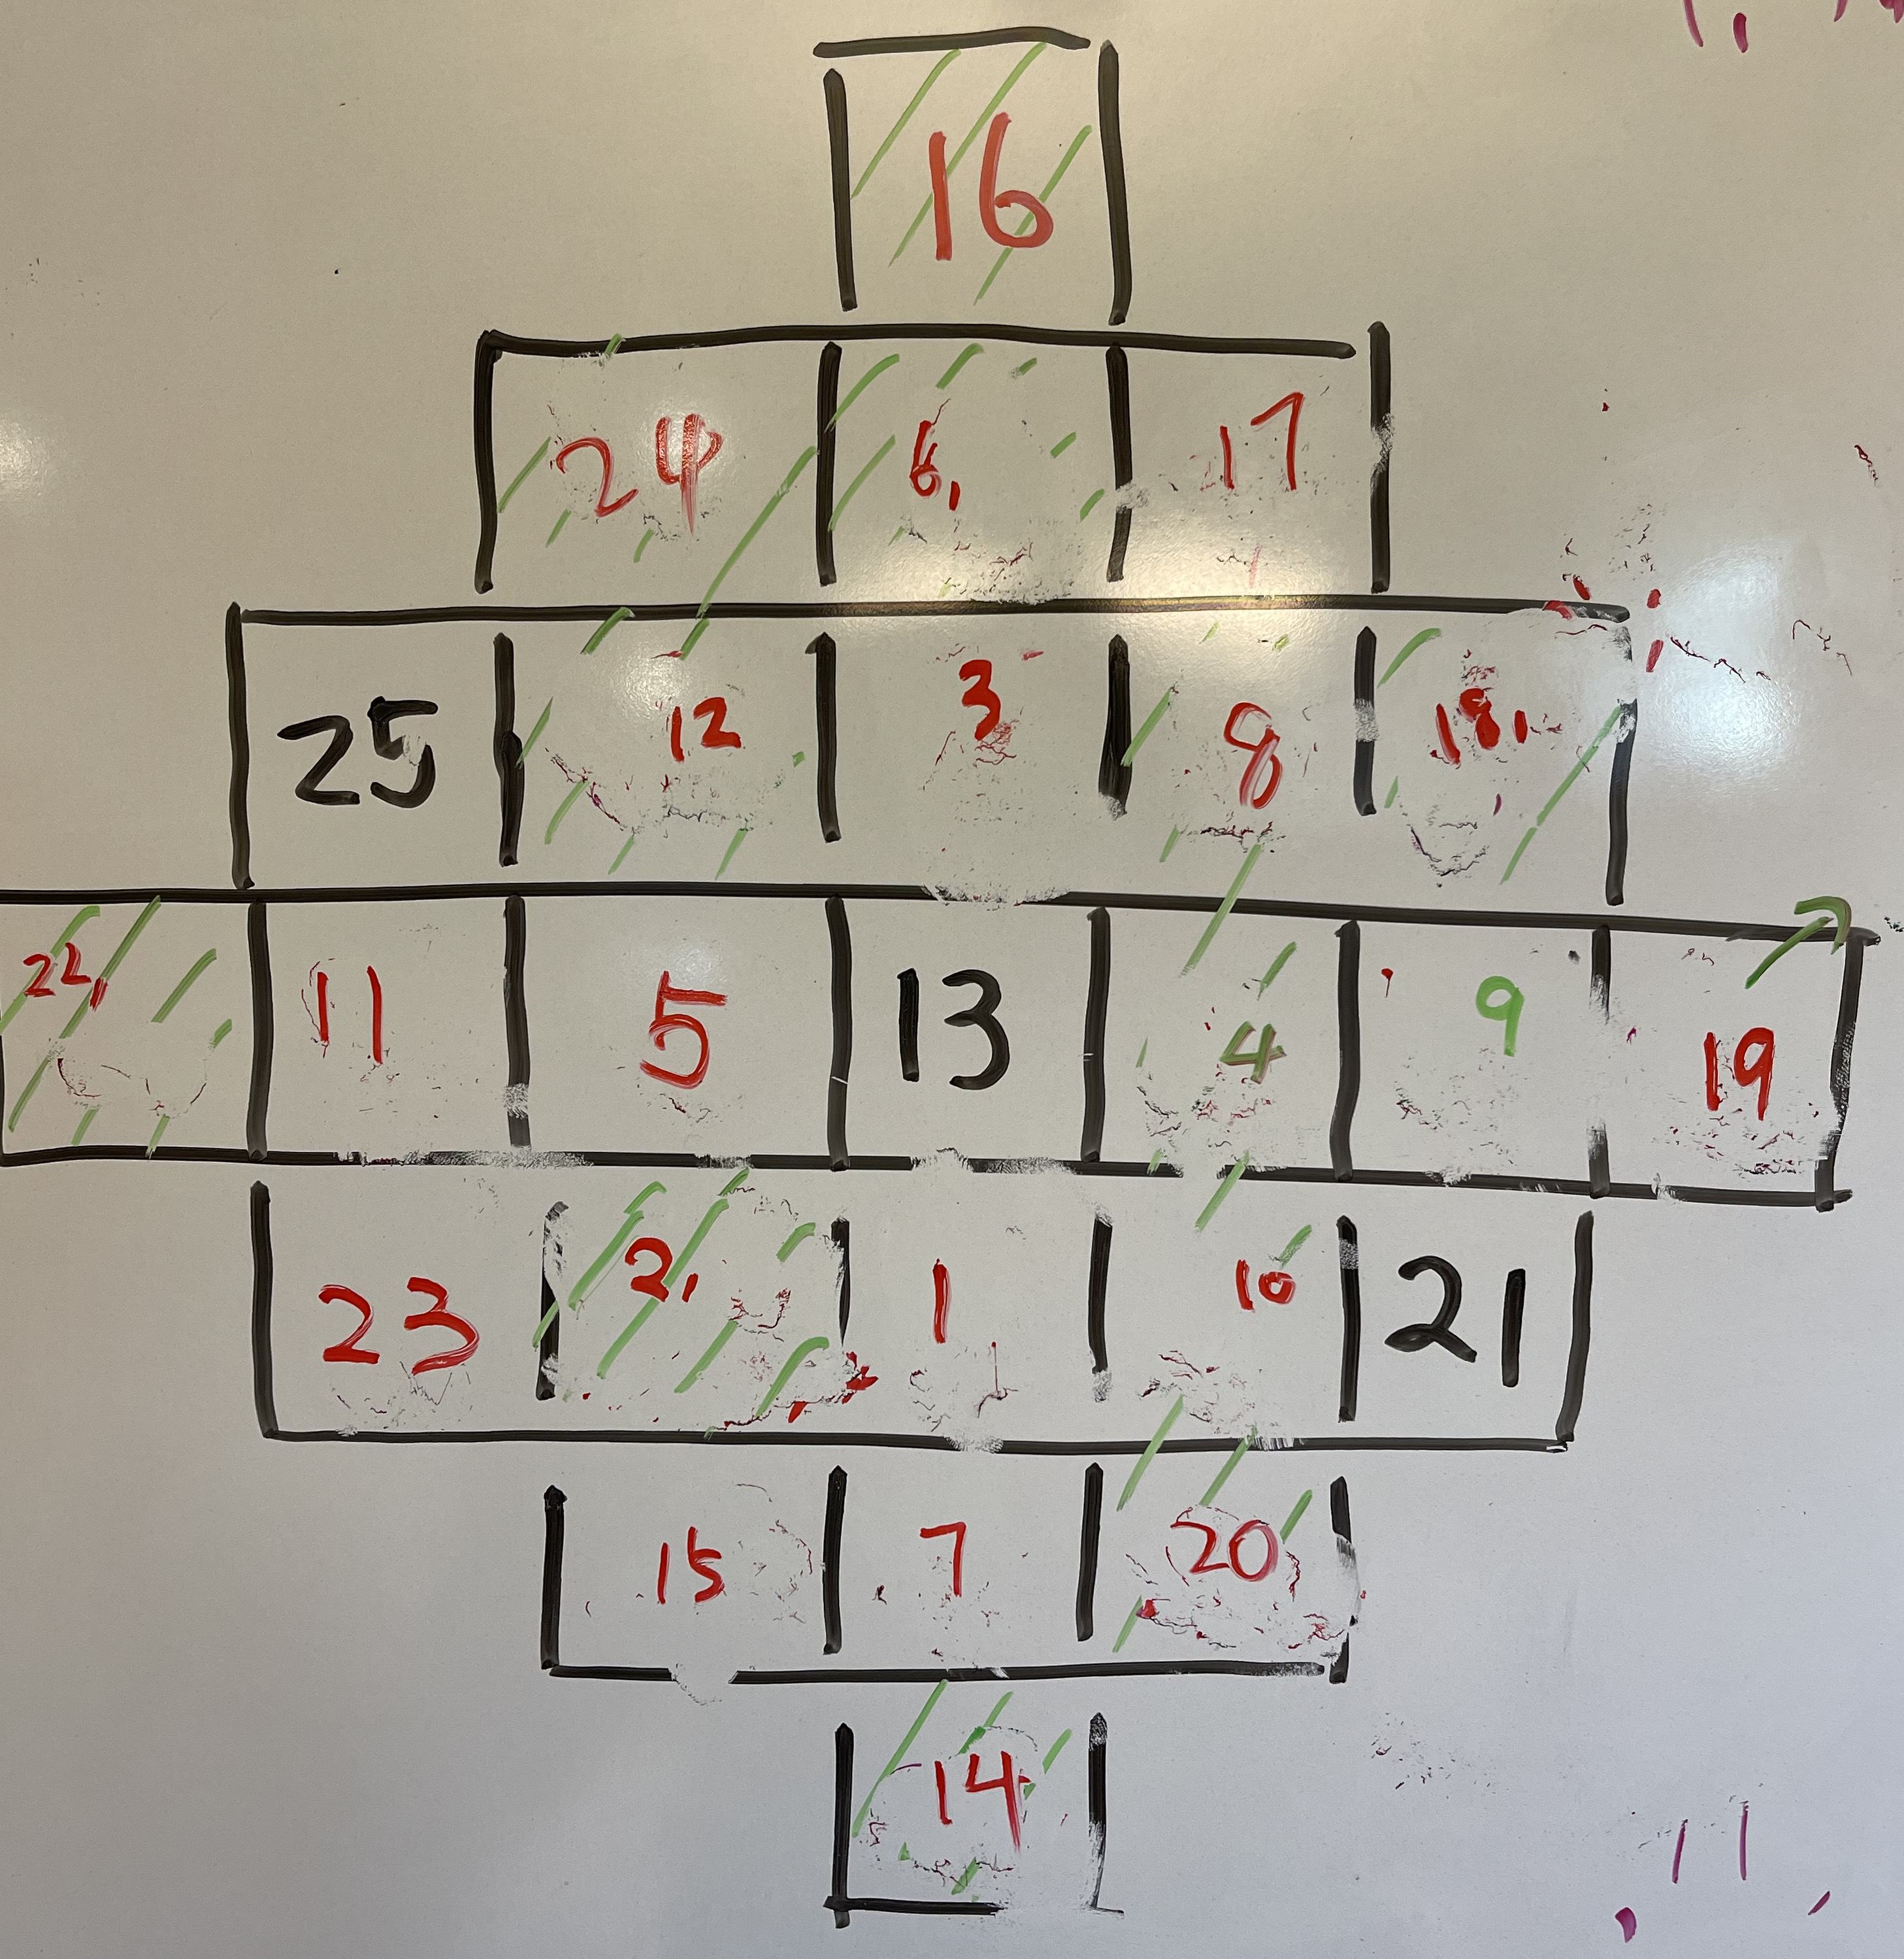
\includegraphics[width=0.7\textwidth]{imgs/p1.png}
%\end{center}
\newpage
\section{Problem 2/2/34}

There are 3 possible outcomes for Grogg: 
\begin{enumerate}
\item He eats 0 cookies, and the probability is $(1-p)$.
\item He eats 1 cookie, and the probability is $p(1-n p^{n-1}(1-p))$.
\item He eats 2 cookies, and the probability is $n p^n (1-p)$.
 \end{enumerate}
 
 The expectation is
 \begin{align*}
& 0\cdot(1-p) +1\cdot p\left(1-n p^{n-1}(1-p)\right) +2\cdot n p^n (1-p)\\
= \quad & p + np^n (1-p).
 \end{align*}
 
 To make the expected value exactly 1, we have
 \begin{align*}
 &p + np^n (1-p)=1\\
 \Rightarrow \quad &np^n(1-p)=1-p, \quad (0<p<1, 1-p \ne 0)\\
 \Rightarrow \quad &np^n=1\\
 \Rightarrow \quad &p=\frac{1}{\sqrt[n]{n}}
 \end{align*}
 
 This is possible for all positive integer $n\ge 2$, where $p=\frac{1}{\sqrt[n]{n}}$. Specifically, when $n=2$, $p=\frac{\sqrt{2}}{2}$.
 
 
 
 \newpage
 \section{Problem 3/2/34}
 
We claim that Lizzie can win the game for any positive composite number $n\ge 4$, and Lizzie can not win the game for any prime number $n\ge 3$.
\begin{proof}
We give the proof in two steps:
\begin{enumerate}
\item We show that Lizzie can win the game for any positive composite number $n\ge 4$. Let $n=ab$, where $ a, b\ge 2, a, b\in \mathbb{Z^+}$. Lizzie can first divide the $n$ numbers into $a$ groups, each of which has $b$ numbers. Lizzie calculate the average of each group and replace numbers in each group with their corresponding averages. Assume the average for group $i$ $(1\le i \le a)$ is $x_i$, Lizzie can then regroup the $n$ numbers into $b$ groups, each of which has $a$ numbers $x_1, x_2,\cdots, x_a$. Taking the average of each of the $b$ groups, Lizzie successfully replaces every number with the average $\frac{1}{a}\cdot\sum^a_{i=1} x_i$.

\item We show that Alex always have a way to make Lizzie lost the game for any prime number $n\ge 3$. First of all, we have to notice that if Lizzie wins the game, the final average should be the mean of all $n$ numbers. This is because Lizzie doesn't change the sum of the group that she is taking the average for. No matter how many times Lizzie takes average and replaces numbers of any subset of the $n$ numbers, the sum of the $n$ numbers remains the same. If at some point Lizzie manages to make the $n$ numbers equal to $k$, then $nk$ should be the sum of the original $n$ numbers, and therefore, $k$ is the mean of the original $n$ numbers.

For any prime number $n\ge 3$, if Alex chooses $n$ numbers such that their sum equals $n+1$, where there are $(n-1)$ 1s and a 2,  then Lizzie will never win the game. Because Lizzie has to make every number $\frac{n+1}{n}$ to win the game. When Lizzie picks some numbers to take average, she has to choose $m$ numbers, where $m<n$. When she takes the average of the $m$ numbers, the average should be $\frac{m+1}{m}$ or $1$.  Suppose Lizzie gets an average of $a_i$ at the $i$-th time, we have that $a_i=1$ or $a_i=\frac{y_i}{x_i}$, where $x_i$ is a product of integers ranging from 2 to $n-1$. $\frac{y_i}{x_i}$ can never be simplified to $\frac{1}{n}$. Therefore, Lizzie can never get the average of $\frac{n+1}{n}$ to win the game.
\end{enumerate}

\end{proof}




 \newpage
 \section{Problem 4/2/34}


The smallest positive integer $c_k=4$, when $k=2$.
\begin{proof}

When $k=2$, lattice points $(x, y)$ and $(x+2, y+2)$ must be the same color according to condition 2. We can color all lattice points with 4 different colors: black, green, blue, and red. For point $(0, 0)$, we color it red. For the neighboring points $(1, 0), (1, 1), (0, 1)$, we color them with blue, green, and black, respectively. In summary, for all the lattice points $(2i, 2j)$ we color red; for all points $(2i+1, 2j)$ we color blue; for all points $(2i+1, 2j+1)$ we color green; for all points $(2i, 2j+1)$ we color black, where $i, j \in \mathbb{Z}$.

We claim that for any $k\ge 3$, we must have $c_k\ge 4$ colors. We derive a coloring scheme in 2 steps.

Step 1: To satisfy condition 1, we first have 4 colors to color all lattice points,  in the same way of what we did for $k=2$. 

Step 2: Given any two lattice points $(x, y)$ and $(a, b)$ such that $x\equiv a \pmod k$ and $y\equiv b \pmod k$.  We have 2 cases: 
\begin{enumerate}
\item $(x, y)$ and $(a, b)$  are colored with the same color in step 1. In this case, condition 2 is satisfied, $c_k=4$.

\item $(x, y)$ and $(a, b)$ are colored with different colors in step 1. To make their colors the same, without violating condition 1, we have to color them with a new color. This is because we can always find a lattice point $t = (x+c, y+d)$, where $c=2\cdot \lfloor\frac{a-x}{2}\rfloor, d=2\cdot \lfloor\frac{b-y}{2}\rfloor$, such that $t$ is a neighboring point of $(a, b)$. By condition 1, $t$ should be different in color from $(a, b)$. By condition 2, $(x, y)$ should be in the same color. Therefore, $(x, y)$ and $(a, b)$ should be colored with a new color to make sure $t$ is NOT in the same color as that of $(x,y)$, and thus $c_k> 4$. 


\end{enumerate}

From the above discussion, we have $c_k\ge 4$ for $k\ge 3$.





\end{proof}






\end{document}  